% Group: 	2
% Name: 	Coding Pharaohs
% Document: 	 Minutes of the third client meeting
% Author:	JianQiu Li
% Date:		Monday August 26 2013

\documentclass[12pt, a4paper]{article}
\topmargin -1cm
\title{Minutes of the Third Client Meeting}
\author{\textsc{Coding Pharaohs} (Group 2)}
\date{August 26 , 2013}
\usepackage{graphicx}
\begin{document}
\maketitle
\begin{tabbing}
\textbf{Chair}~~~~~~~~\= Bowen Tao   \\
\textbf{Secretary}    \>      Jianqiu Li       \\
\textbf{Members}      \>Yifei Pei             \\
                      \>Matthew Nestor        \\
                      \>  Abdulaziz Alhulayfi    \\
                      \>Yu Hong               \\
\textbf{Apologies}    \>None                  \\
\end{tabbing}
\section{Time and Place}
The third client meeting for Software Engineering and Project was held in \textbf{Ingkarni Wardli, Room 462 \textnormal{at} 2:30pm \textnormal{on} Monday 26 August 2013}.
\section{Quorum Announcement}
Having determined that quorum was satisfied, the Chairman Mr.~Bowen declared the meeting open.
\section{Summary of Previous Meeting}
Yu Hong and JianQiu Li make a description about the prototype of the robot. They explained the function of the prototype of the robot and provided the reason of constructing this prototype. Then, the other group members asked more questions in terms of the functional requirements, such as the the road closure and the information of the map. 
\section{Group Milestone: SRS presentation}
\subsection{Overview}
JianQiu Li made a presenation about SRS document


\subsection{SRS Detailed Presentation}
\begin{itemize}
 \item JianQiu Li summarised the information which from SRS document, this includes the user requirements and some other non-functional requirements. All these information contribute to the system features which are the manual control and the automatic mapping function. 
\end{itemize}

\section{Individual Milestone Report: GUI mockup}
\subsection{Overview}
YiFei Pei showed the GUI to the client
\subsection{GUI Detailed Presentation}
\begin{itemize}
 \item According to the milestone of Week 5, YiFei Pei introduced the GUI mockups. In the presentation, the function of GUI includes 
\\- The GUI contains an area to display the map
\\- some buttons of robot movement controls 
\\- dangerous zone editing
\\- The buttons of map loading and saving
\\- The GUI can display the operator feedback
\\- robot representation
\\- Battery life and bluetooth signal representations on GUI
\end{itemize}
\section{milestone negotiation for Week 9 and 10}

The group submitted the milestone form for Week 9 and Week 10 to the client.

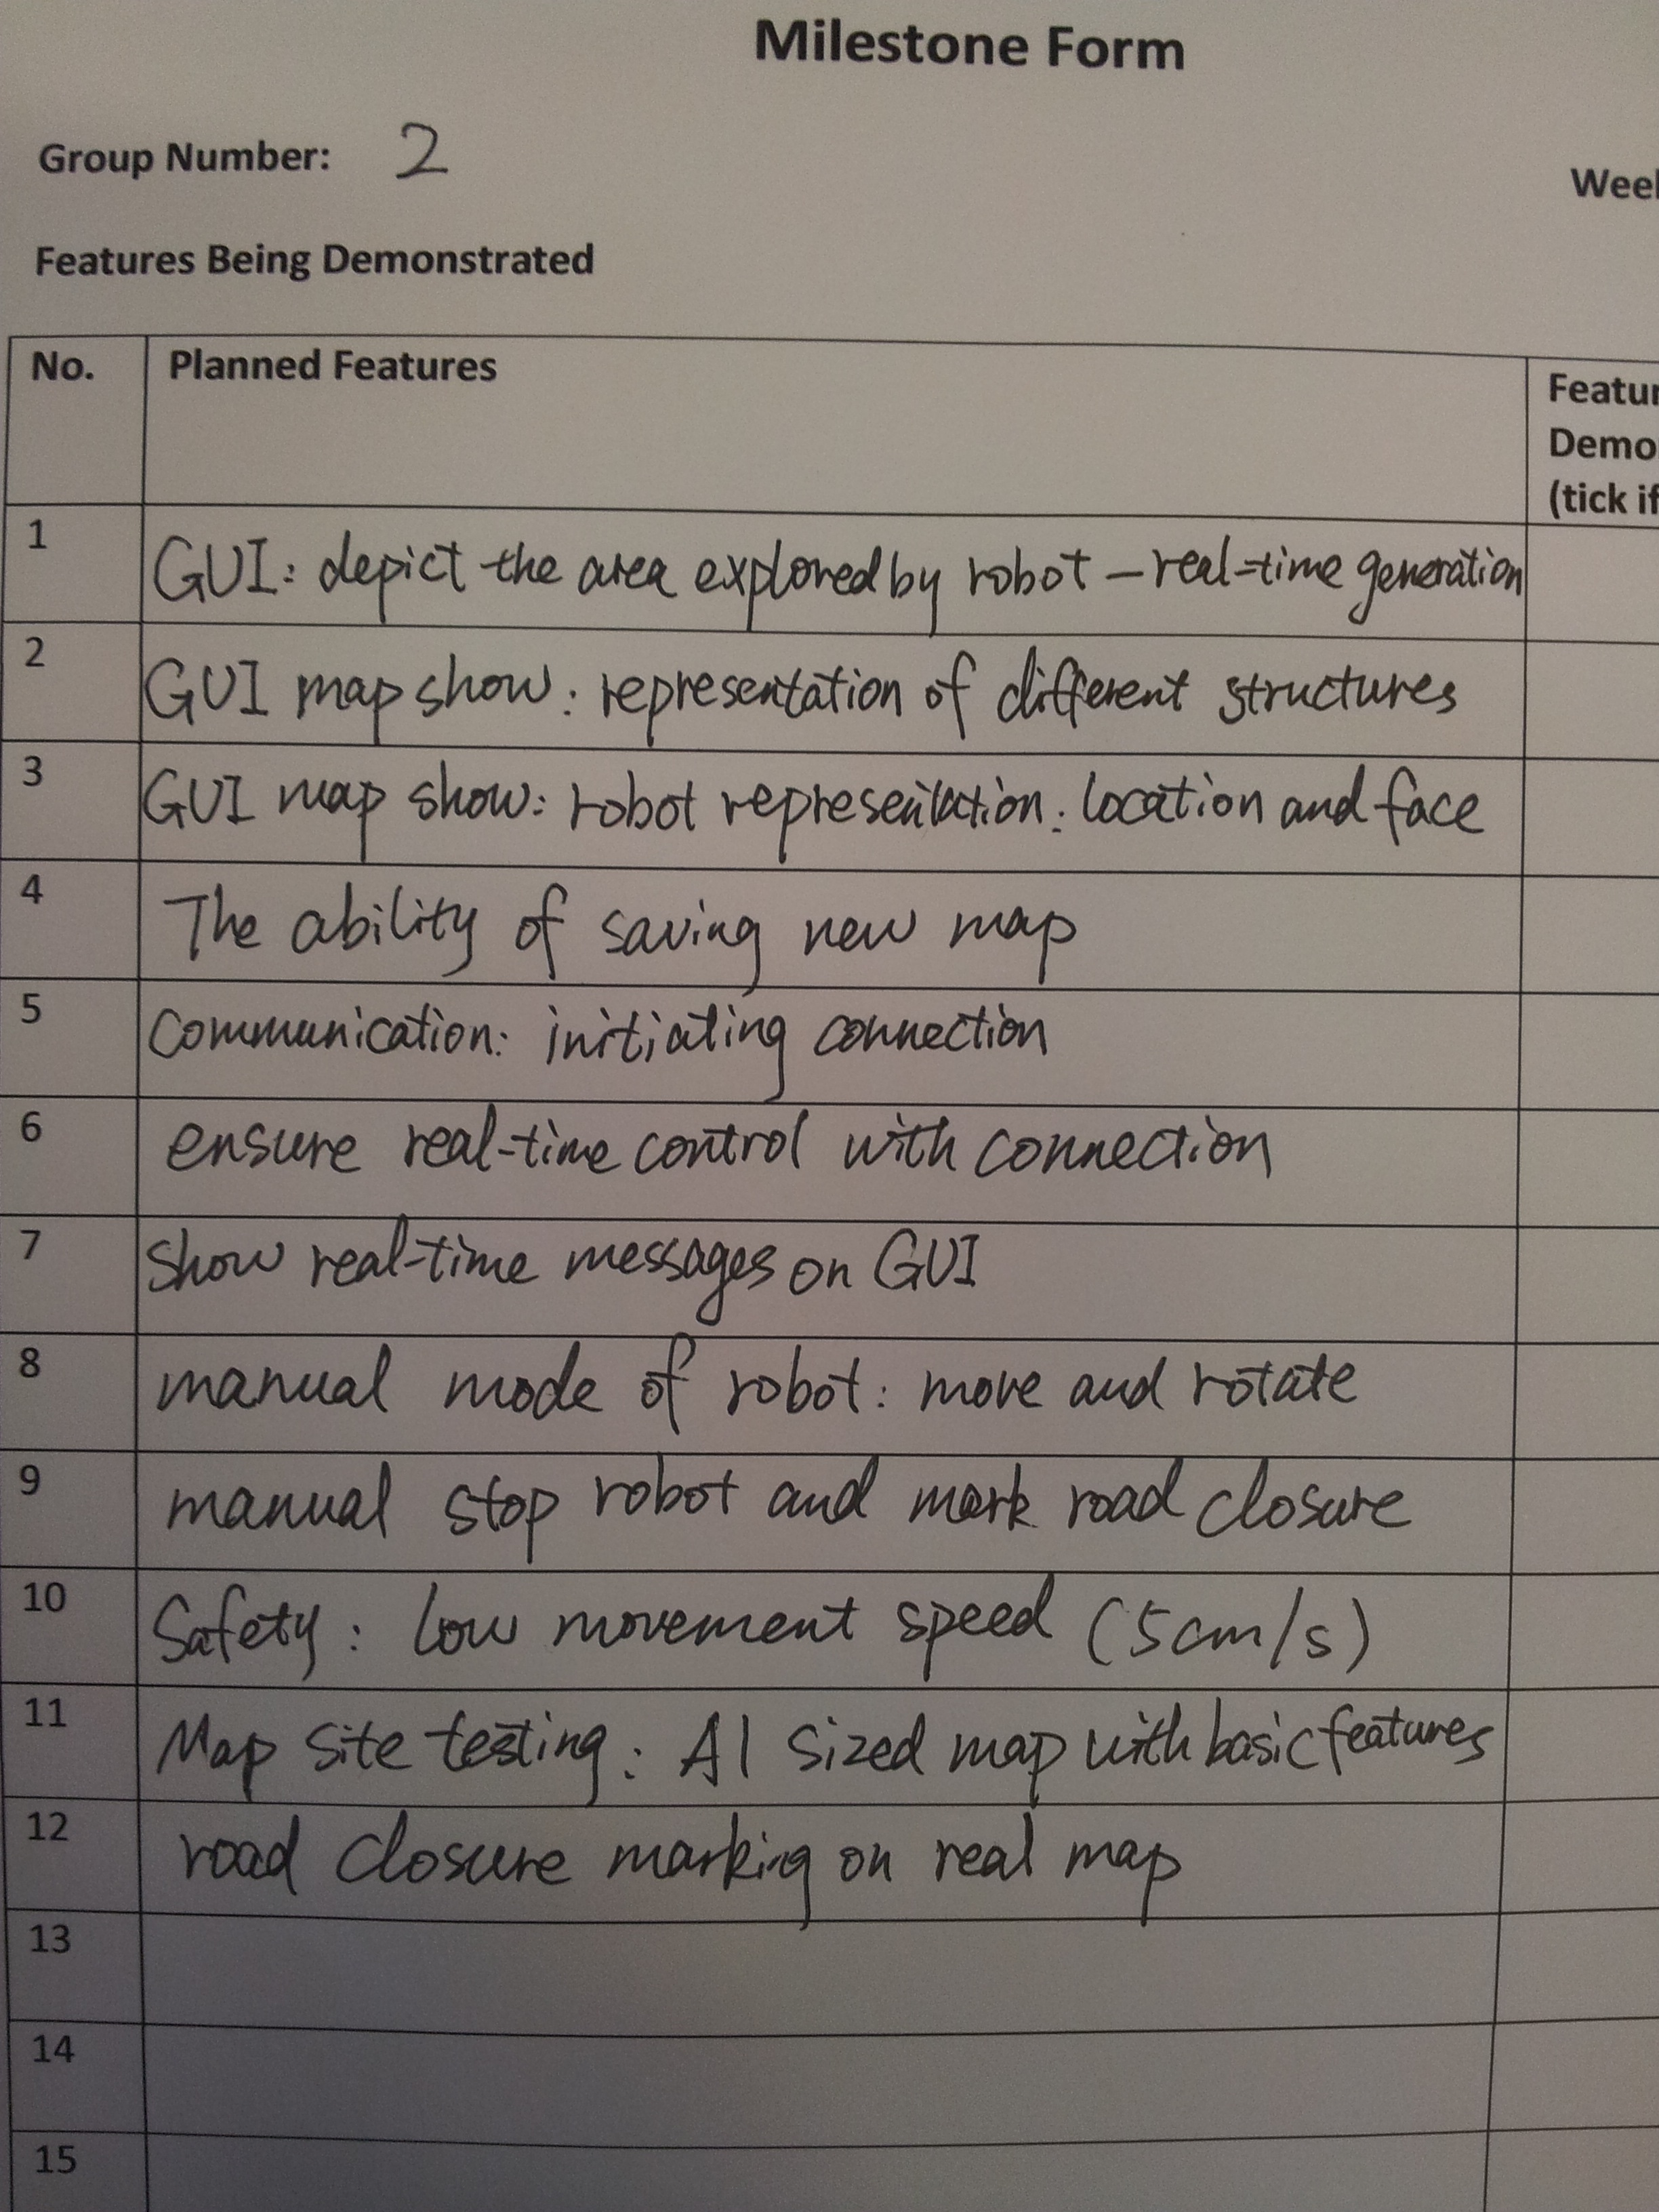
\includegraphics[width=15cm]{/Study/Aus_2013/sep2013-2/individuals/Yifei/appendices/Week9milestoneform.jpg}

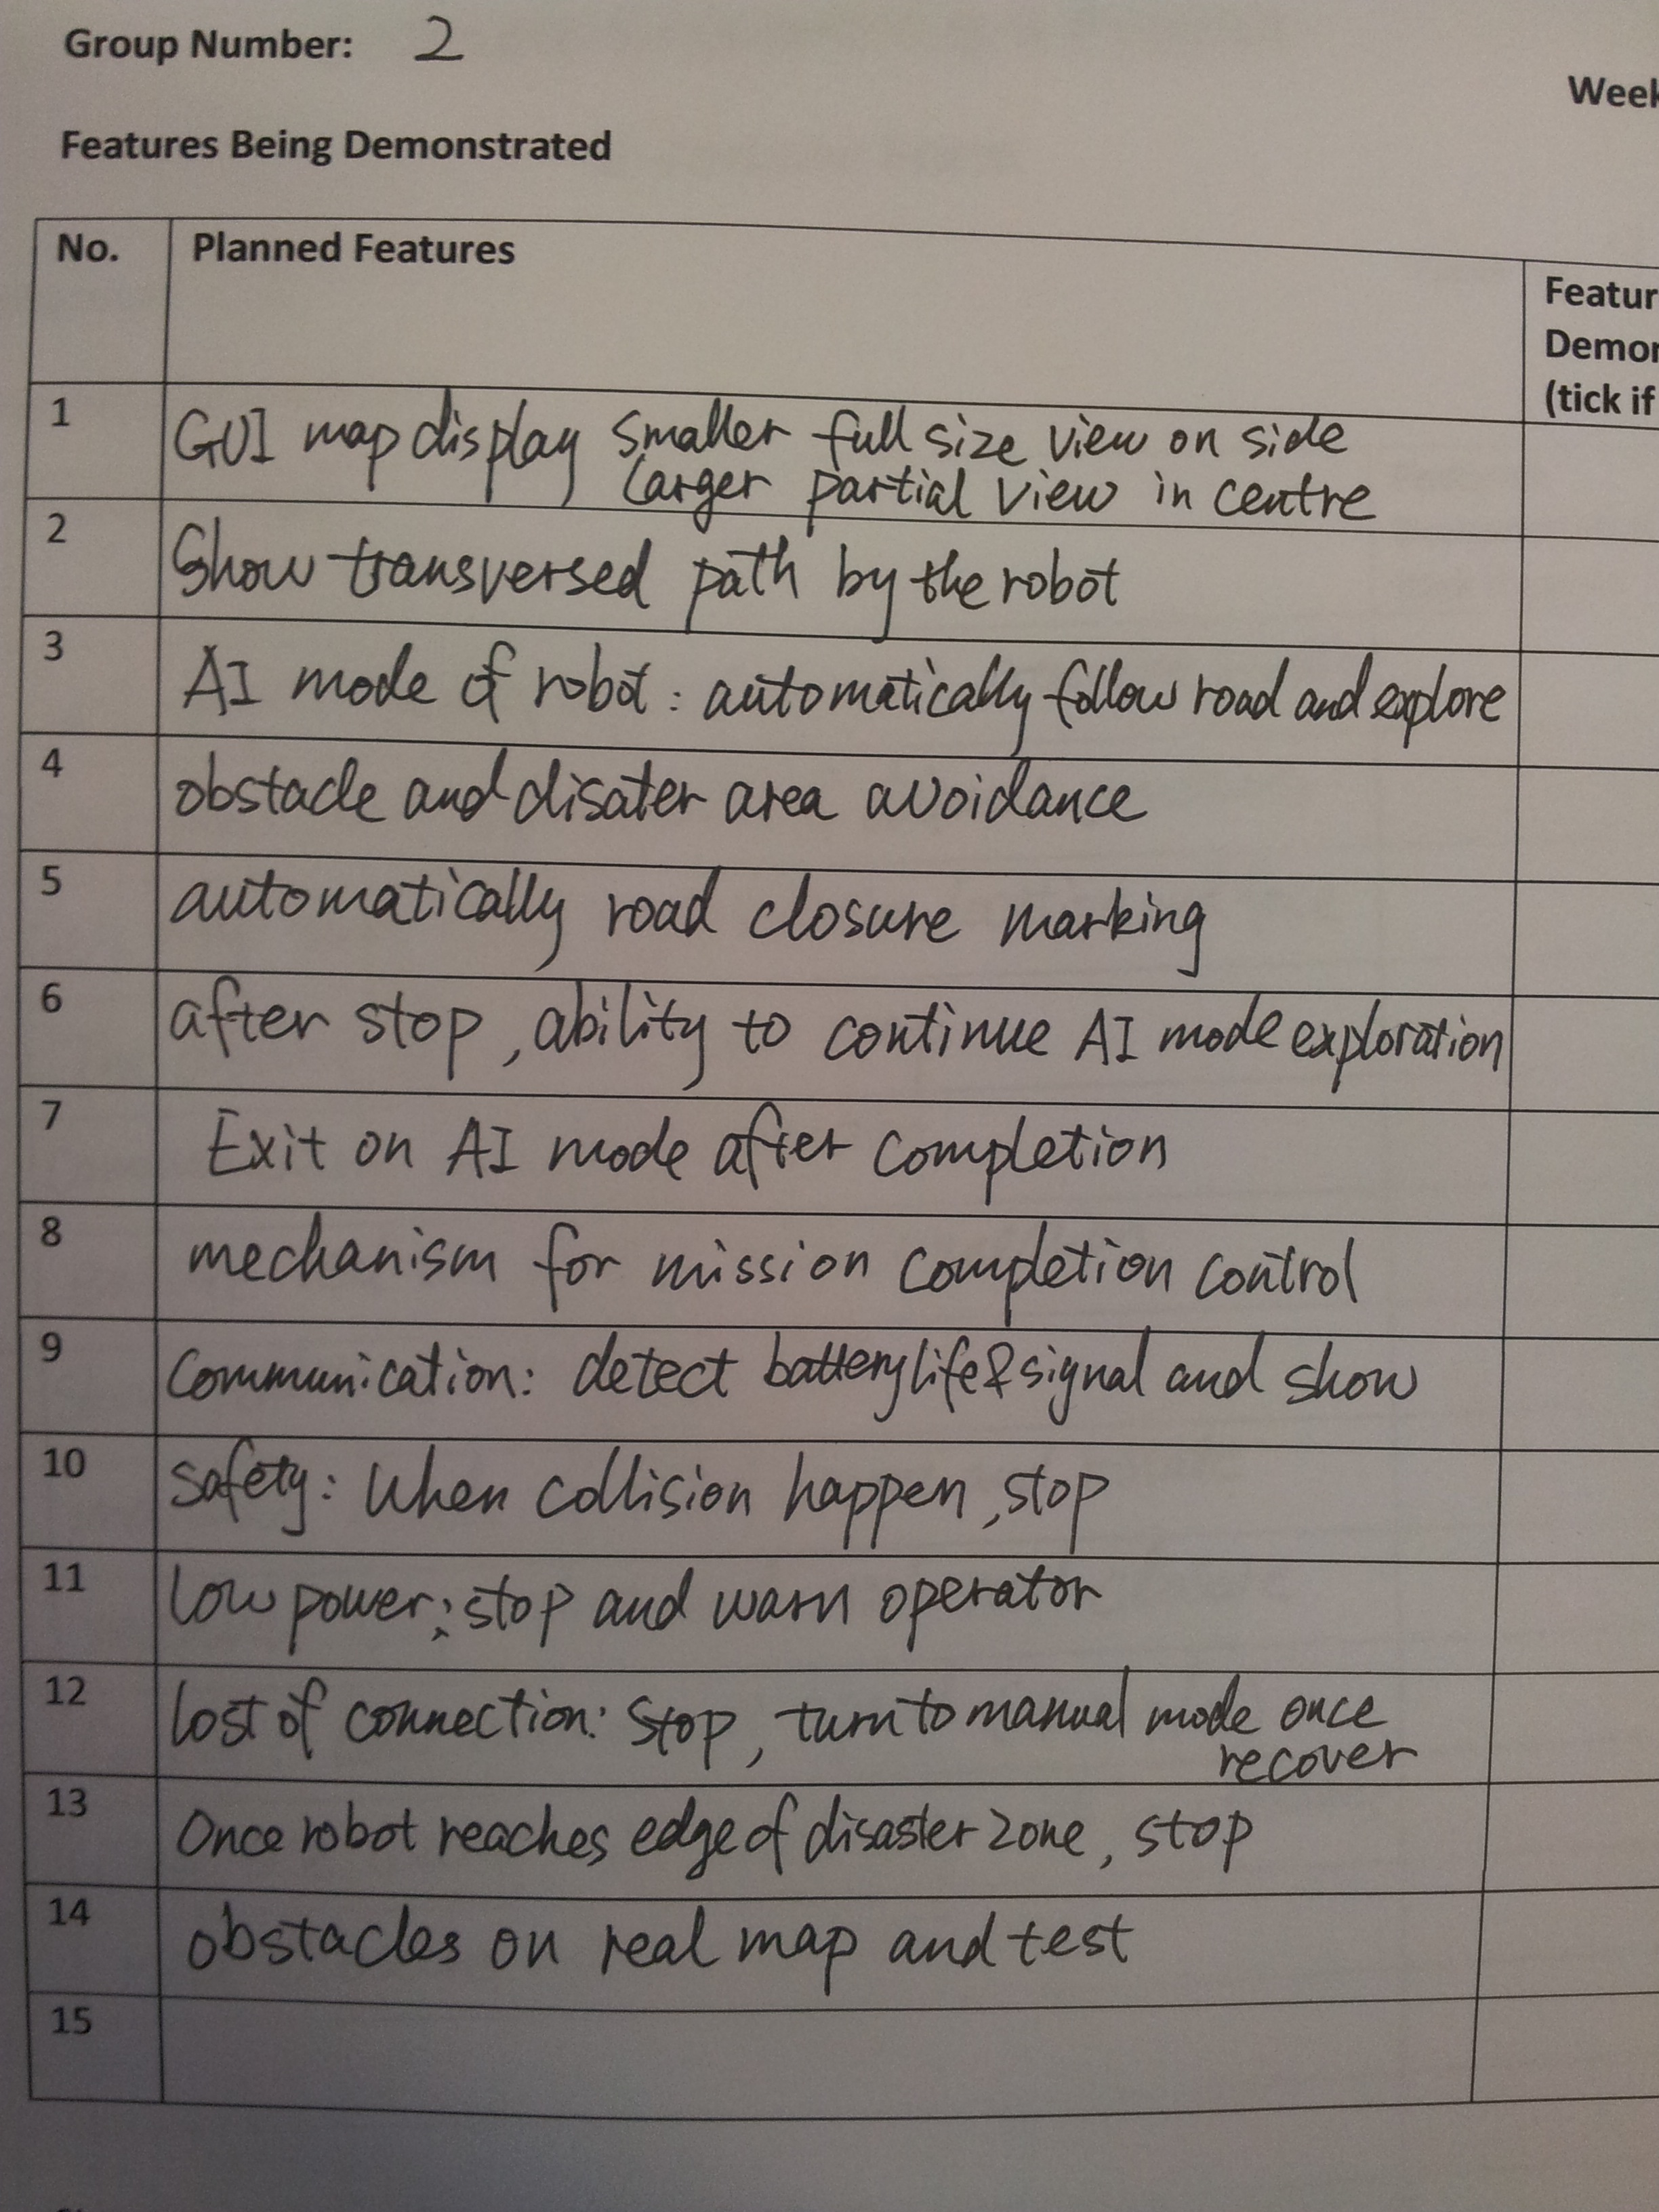
\includegraphics[width=15cm]{/Study/Aus_2013/sep2013-2/individuals/Yifei/appendices/Week10milestoneform.jpg}

\section{Requirements Elicitation}
The majority of the meeting consisted of interviewing the client for project requirements.  A paraphrased summary of the questions, and client answers, follows:

\subsection{Functional Requirements}
\begin{enumerate}
 \item \textbf{Mr.~Nestor:}      From the DTD, the road are perpendicular to each other, Do they have constant turning angles or not?  \\
       \textbf{Client:}     There are many cases in real situtation, we should assume all the condition of the roads. Thus, the road can be any cases, and use line statement on XML. 
 

 \item \textbf{Mr.~Bowen:}     What is the  physical shape of the obstacles and intersections ? how to distinguish them? \\
       \textbf{Client:}     The physical shape of the obstacles should be a cycle and you can use different colours to distinguish them. The robot also need to detect the shape of  obstacles and draw on the map


\end{enumerate}
\section{Meeting Feedback}
The tutor gave the group some feedback for its performance in its third client meeting. The following is a
summary of the key points.
\begin{itemize}
 \item we should prepare details of milestone 9,10 next week that get the feedback
\end{itemize}
\begin{itemize}
 \item we should add the speed button on the GUI which can control the speed of the robot. This is for the emergency cases which can make the robot get the emergency place quickly
\end{itemize}

\begin{itemize}
 \item We should change the size of some buttons, for example the stop button, we need make it more visable 
\end{itemize}

\section{Adjournment}
The next meeting is a group meeting to be held in the same place, namely Ingkarni
Wardli, Room 462 at 2:30pm on Thursday 2 September 2013.\\
The meeting will close around 3:10pm.
\end{document}